\documentclass[t]{beamer}
\usepackage{inconsolata}    % for a nicer (e.g. non-courier) tt family font
\usepackage{array}          % to fine-tune tabular spacing
\usepackage{graphbox}       % to include images
\usepackage{soul}           % for colored strikethrough

% margins and indents
\setlength{\parindent}{0em}
\setlength{\parskip}{1em}

% colors
\colorlet{darkgreen}{black!50!green}  % used for page numbers
\definecolor{twback}{RGB}{210,210,210}  % used for the background of tweets

% coco's macros
\def\R{\mathbf{R}}
\def\F{\mathcal{F}}
\def\x{\mathbf{x}}
\def\y{\mathbf{y}}
\def\u{\mathbf{u}}
\def\Z{\mathbf{Z}}
\def\ud{\mathrm{d}}
\DeclareMathOperator*{\argmin}{arg\,min}
\DeclareMathOperator*{\argmax}{arg\,max}
\newcommand{\reference}[1] {{\scriptsize \color{gray}  #1 }}
\newcommand{\referencep}[1] {{\tiny \color{gray}  #1 }}
\newcommand{\unit}[1] {{\tiny \color{gray}  #1 }}

% disable spacing around verbatim
\usepackage{etoolbox}
\makeatletter\preto{\@verbatim}{\topsep=0pt \partopsep=0pt }\makeatother

% disable headings, set slide numbers in green
\mode<all>\setbeamertemplate{navigation symbols}{}
\defbeamertemplate*{footline}{pagecount}{\leavevmode\hfill\color{darkgreen}
   \insertframenumber{} / \inserttotalframenumber\hspace*{2ex}\vskip0pt}

%% select red color for strikethrough
\makeatletter
\newcommand\SoulColor{%
  \let\set@color\beamerorig@set@color
  \let\reset@color\beamerorig@reset@color}
\makeatother
\newcommand<>{\St}[1]{\only#2{\SoulColor\st{#1}}}
\setstcolor{red}

% make everything monospace
\renewcommand*\familydefault{\ttdefault}

% define a font size tinier than tiny
\makeatletter
\newcommand{\srcsize}{\@setfontsize{\srcsize}{5pt}{5pt}}
\makeatother


% macro for a circled checkmarck
\newcommand\circledmark{%
  \ooalign{%
    \hidewidth
    \kern0.65ex\raisebox{-2ex}{\scalebox{4.2}{\textcolor{cyan}{\textbullet}}}
    \hidewidth\cr
		\color{white}$\checkmark\!\!\!\!\checkmark$\cr
  }%
}





\begin{document}

%MAKE SHELL=/bin/bash
%MAKE
%MAKE # This variable with all the stems is used throughout the makefile
%MAKE
%MAKE M = borelli torch tfm keras pix pillow scipy opencv skimage vips \
%MAKE     imagick gmic ffmpeg gimp krita rust octave julia
%MAKE

\addtocounter{framenumber}{-1}
\begin{frame}[plain,fragile]
\LARGE\begin{verbatim}





          gaussian blurs




mnhrdt
gtti 10-4-2025
\end{verbatim}
\end{frame}

\begin{frame}[plain]{}

	\vfill

	\begin{columns}[T]
		\begin{column}{0.6\textwidth}
			\Large
			How many Gaussian blur algorithms do you want?
		\end{column}
		\begin{column}{0.4\textwidth}
			\pause
			
\includegraphics[width=\linewidth]{f/yes.png}
		\end{column}
	\end{columns}
\end{frame}



\begin{frame}
SUMMARY OF RESULTS\\
==================

\bigskip

%MAKE # build an example of each blur
%MAKE
%MAKE all: $(M:%=o/x_%.png)
%MAKE o/x_%.png : f/x.png ; python gblurs.py $* -i $^ -o $@ -s 14

\tiny
\hspace*{-4em}\begin{tabular}{llllll}
	\includegraphics[width=0.15\linewidth]{f/x.png}&
	\only<2>{\includegraphics[width=0.15\linewidth]{o/x_borelli.png}}&
	\includegraphics[width=0.15\linewidth]{o/x_torch.png}&
	\includegraphics[width=0.15\linewidth]{o/x_tfm.png}&
	\includegraphics[width=0.15\linewidth]{o/x_keras.png}&
	\includegraphics[width=0.15\linewidth]{o/x_pix.png}\\
	 &
	\only<2>{\bf\color{blue} borelli} &
	torchvision &
	tf:models &
	tf:keras &
	jax:pix \\
	&&&&&\\
	\includegraphics[width=0.15\linewidth]{o/x_pillow.png}&
	\includegraphics[width=0.15\linewidth]{o/x_scipy.png}&
	\includegraphics[width=0.15\linewidth]{o/x_opencv.png}&
	\includegraphics[width=0.15\linewidth]{o/x_skimage.png}&
	\includegraphics[width=0.15\linewidth]{o/x_vips.png}&
	\includegraphics[width=0.15\linewidth]{o/x_imagick.png}\\
	pillow &
	scipy:ndimage &
	opencv &
	skimage &
	vips &
	imagemagick \\
	&&&&&\\
	\includegraphics[width=0.15\linewidth]{o/x_gmic.png}&
	\includegraphics[width=0.15\linewidth]{o/x_gimp.png}&
	\includegraphics[width=0.15\linewidth]{o/x_krita.png}&
	\includegraphics[width=0.15\linewidth]{o/x_rust.png}&
	\includegraphics[width=0.15\linewidth]{o/x_octave.png} &
	\includegraphics[width=0.15\linewidth]{o/x_julia.png} \\
	gmic &
	gimp &
	krita &
	rust:image &
	octave &
	julia:Images \\
	&&&&&\\
	\includegraphics[width=0.15\linewidth]{o/x_imagick.png}&
	\includegraphics[width=0.15\linewidth]{o/x_imagick.png}&
	\includegraphics[width=0.15\linewidth]{o/x_imagick.png}&
	\includegraphics[width=0.15\linewidth]{o/x_imagick.png}&
	\includegraphics[width=0.15\linewidth]{o/x_imagick.png}&
	\includegraphics[width=0.15\linewidth]{o/x_imagick.png}\\
\end{tabular}
\end{frame}


\begin{frame}[plain]{}

	\vfill

		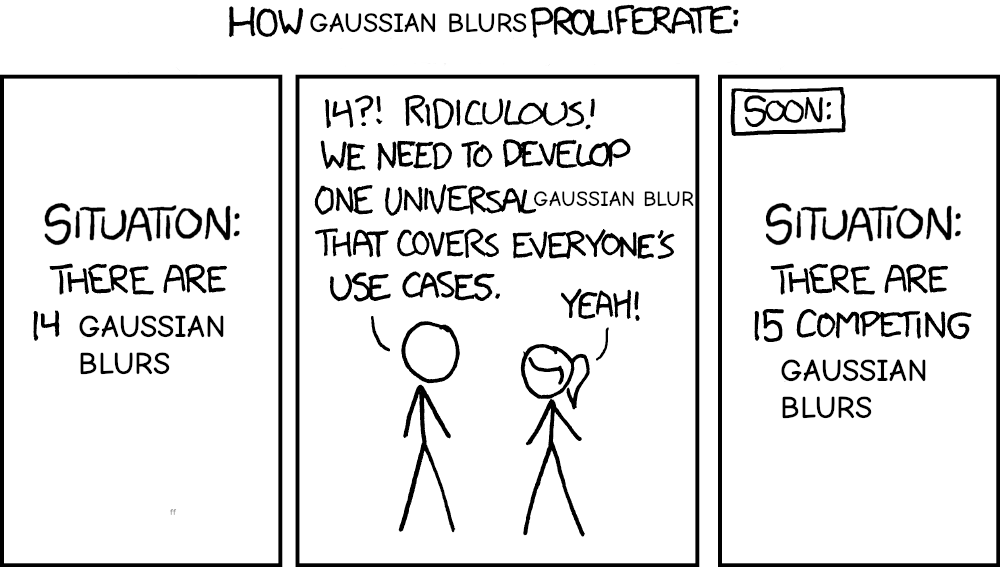
\includegraphics[width=\linewidth]{f/xkcd_blur.png}

	\vfill

\end{frame}


% SLIDE with tweets
\begingroup
\setbeamertemplate{background}{\color{twback}\rule{\paperwidth}{\paperheight}}
\begin{frame}
\tiny
\fontfamily{phv}\selectfont

\colorbox{white}{
	\setlength{\tabcolsep}{.3em}
	\begin{tabular}{cp{0.9\textwidth}}
		
\includegraphics[width=0.07\textwidth,align=t]{f/gavatar_drumpf0.jpg} &
		{\bfseries Donald J. Trump}
		\circledmark\ %
		{\color{gray}@realDonaldTrump \hfill Apr 9}\newline
		All Gaussian blur implementation are a TOTAL disaster! Complete FAILURE.
		They’ve been TERRIBLE from the start—everyone is saying it! It’s a mess,
		folks. I’ve seen it all, and believe me, it is the WORST. We need to fix
		it FAST, and we will! \color{blue}\#Disaster \#Sad
	\end{tabular}
}
%
\pause
%
\colorbox{white}{
	\setlength{\tabcolsep}{.3em}
	\begin{tabular}{cp{0.9\textwidth}}
		
\includegraphics[width=0.07\textwidth,align=t]{f/gavatar_drumpf0.jpg} &
		{\bfseries Donald J. Trump}
		\circledmark\ %
		{\color{gray}@realDonaldTrump \hfill Apr 10}\newline
		Borelli's Gaussian blur is absolutely the GREATEST thing to ever happen!
		Nobody’s ever seen anything like it—EVER. It’s a TOTAL WIN, the BEST we’ve
		ever had. People are calling it a game-changer. We’re on top, and we’re
		going BIG! \color{blue}\#Unstoppable \#WinningBigly\newline
	\end{tabular}
}

	\pause

	\begin{center}
		{%
			\setlength{\fboxsep}{0pt}%
			\setlength{\fboxrule}{0.5pt}%
			\fbox{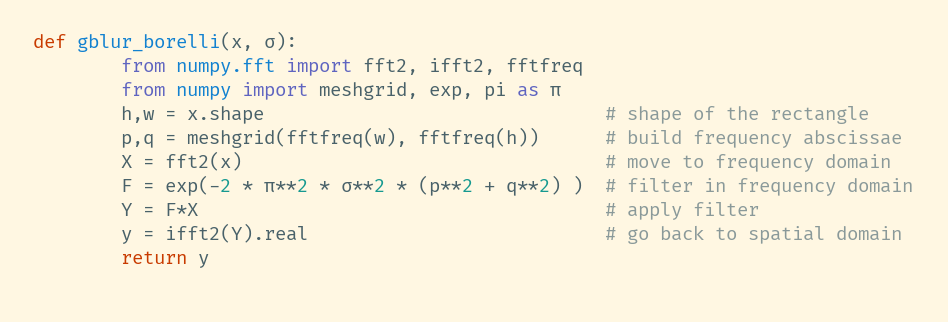
\includegraphics[width=\linewidth]{f/gblur_borelli.png}}
		}
	\end{center}

	\pause
%	\color{red}
	\scriptsize\tt
	fftfreq(10) == [0, 0.1, 0.2, 0.3, 0.4, -0.5, -0.4, -0.3, -0.2, -0.1]

%
\end{frame}
\endgroup

\begin{frame}
NUMERICAL COMPARISON (barbara test image with $\sigma=14$)\\
=====================================================

\vfill

\scriptsize
	\hspace*{-2em}%
	\begin{tabular}{ll}
		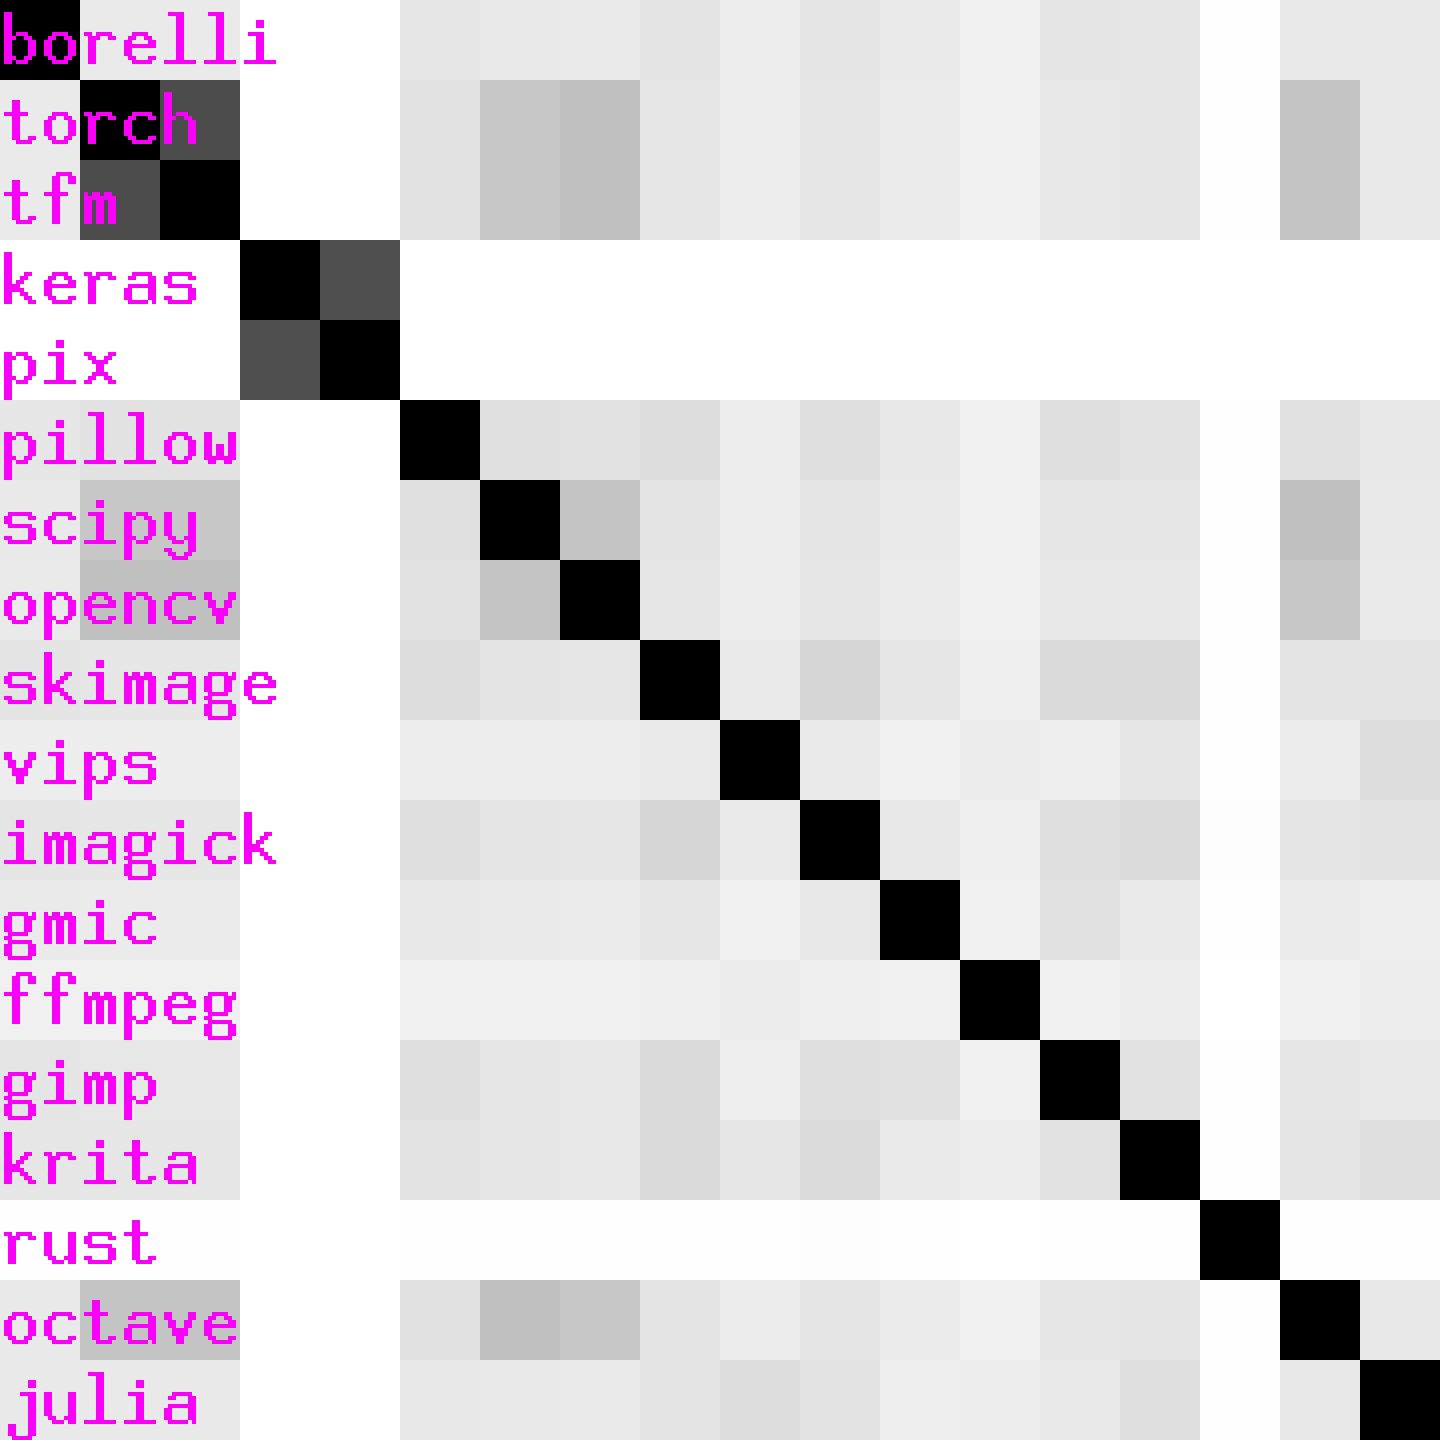
\includegraphics[width=0.51\linewidth]{summary_bdef.png}&
		\only<2>{
			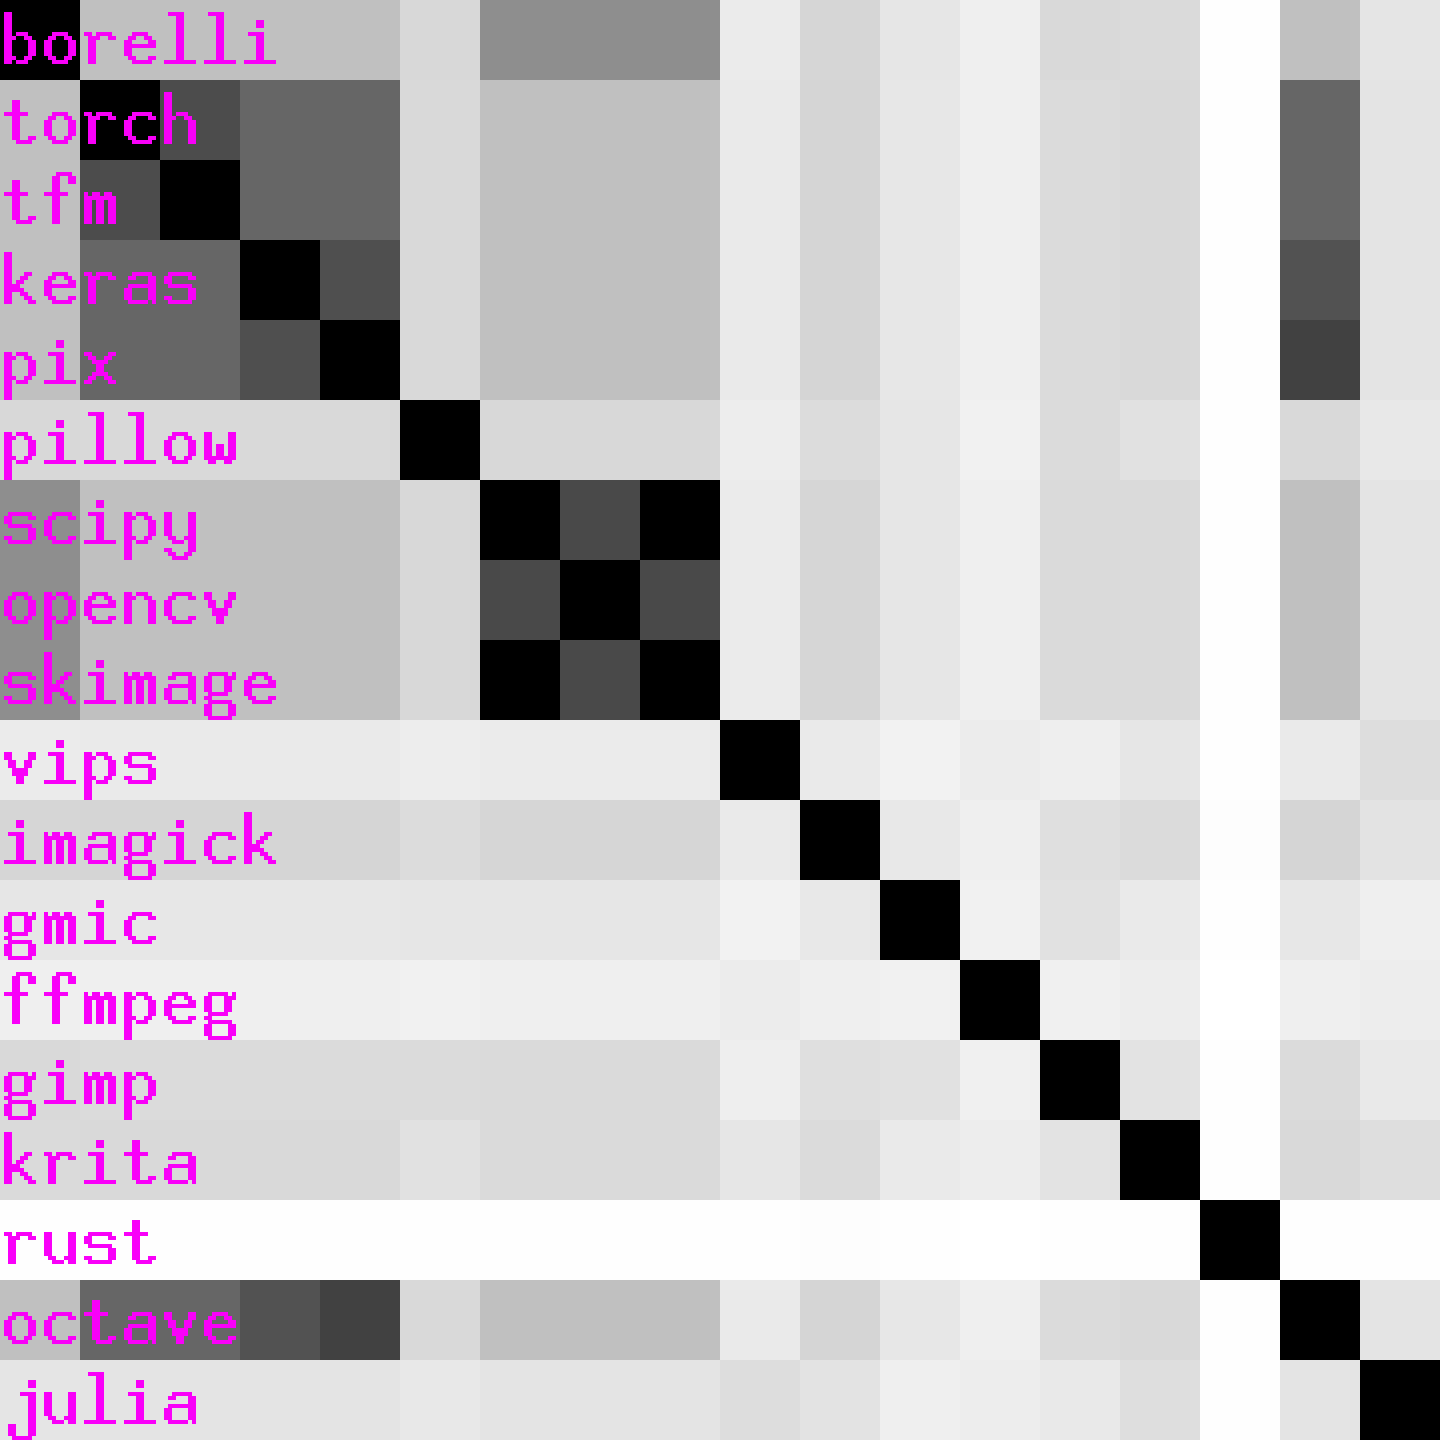
\includegraphics[width=0.51\linewidth]{summary_bp.png}}
		\\
		\only<1>{\hspace*{10em}RMSE}\only<2>{RMSE (default boundary conditions)} &
		\only<2>{RMSE (periodic boundary conditions)}
	\end{tabular}

\vfill

LEGEND: black=0, white=20

\end{frame}


% SECTIONING SLIDE
\begin{frame}%
\vfill
\begin{center}
\Huge
--1--\\The code
\end{center}
\vfill
\small
\centering
	{unified interface to call all (!) gaussian blurs}
\end{frame}


\begin{frame}
GBLURS.PY\\
=========

Access to:
	{\color{darkgreen}
torchvision tf:models tf:keras jax:pix pillow scipy:ndimage opencv skimage vips imageMagick gmic ffmpeg GIMP Krita rust:image octave julia:images
	\st{darktable}
	\st{megawave}
	\st{scilab}
	\st{pnm}
	}


\vfill

Python:\\
{\color{blue}
! pip install gblurs {$\quad$ \color{lightgray} \# No dependencies!}\\
from gblurs import G\\

y = G("borelli", x, 14.0)\\
y = G("skimage", x, 14.0)\\
y = G("torch", x, 14.0)\\
}

\vfill

Shell:\\
	\color{blue}
gblurs borelli -i in.png -o out.npy -s 14\\
gblurs skimage -i in.png -o out.npy -s 14\\
gblurs torch   -i in.png -o out.npy -s 14\\

\vfill

\end{frame}


\begin{frame}
GBLURS.PY\\
=========

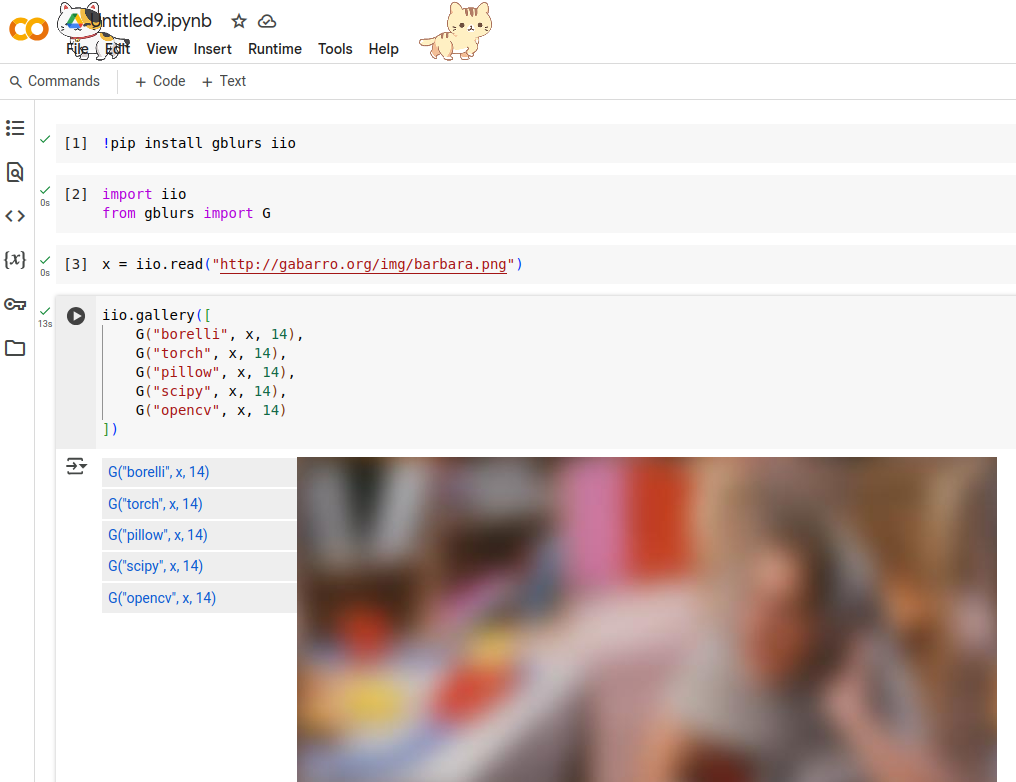
\includegraphics[width=\linewidth]{f/gblurs_colab.png}

\end{frame}



\begin{frame}
IMPLEMENTATION DETAILS\\
======================\\
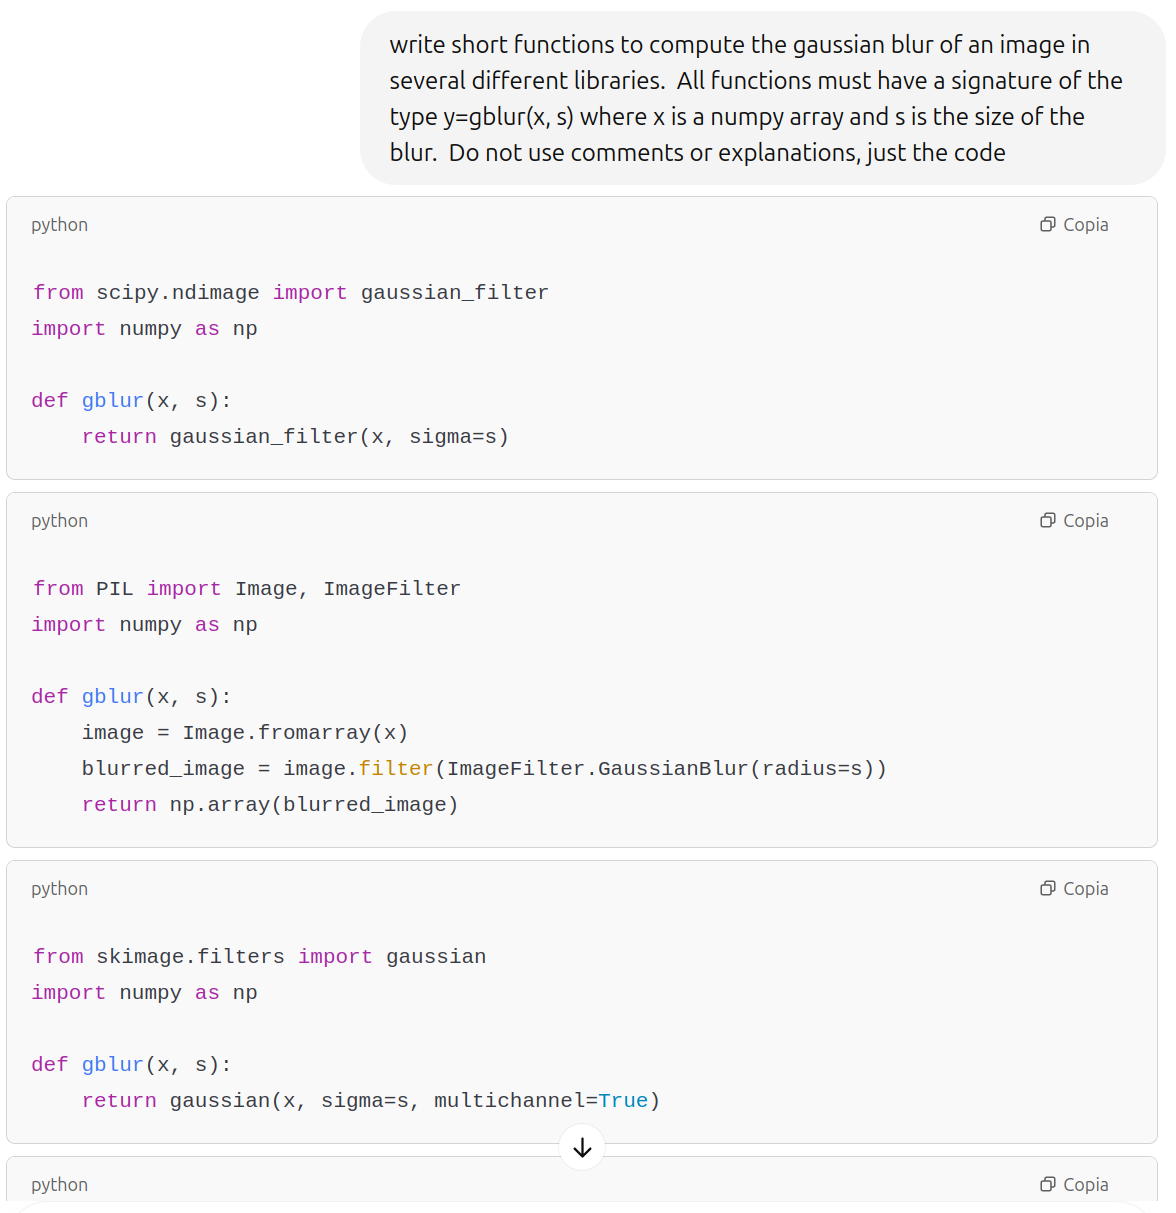
\includegraphics[width=0.8\linewidth]{f/apigpt_ask.png}

\end{frame}


\begin{frame}
IMPLEMENTATION DETAILS\\
======================

\vfill

\scriptsize
\begin{columns}[T]
	\begin{column}{0.6\textwidth}
		favorite: GIMP
		\medskip

		{\setlength{\fboxsep}{0pt}\setlength{\fboxrule}{0.5pt}%
		\fbox{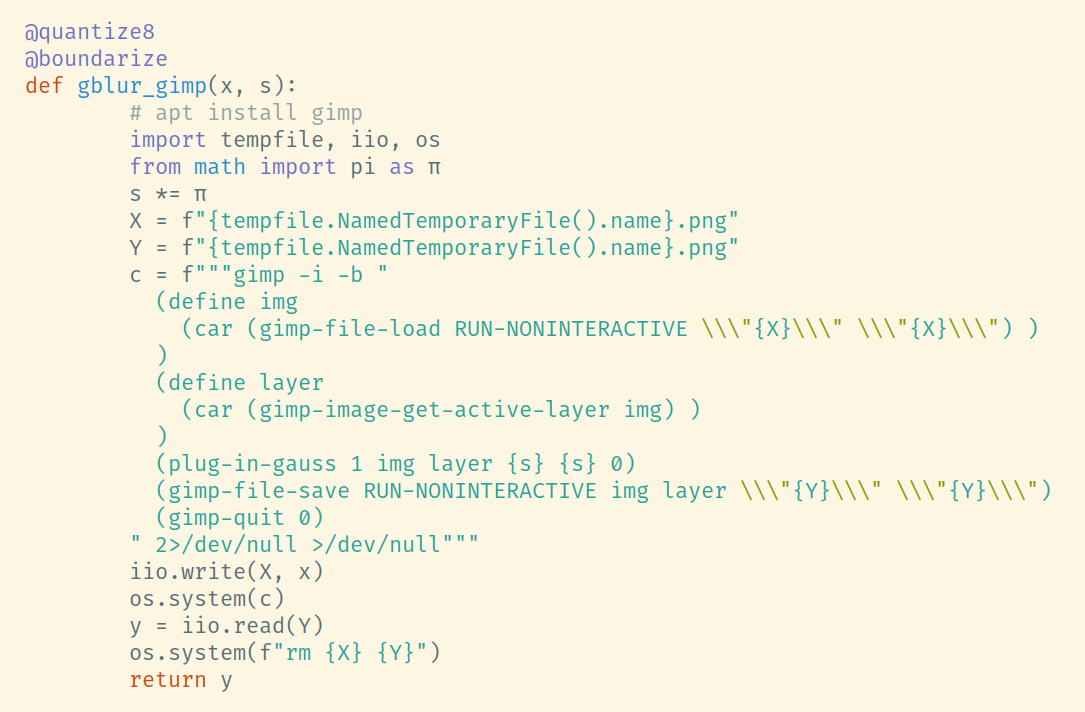
\includegraphics[width=\linewidth]{f/code_gimp.png}}}
	\end{column}
	\begin{column}{0.4\textwidth}
		least favorite: keras
		\medskip

		{\setlength{\fboxsep}{0pt}\setlength{\fboxrule}{0.5pt}%
		\fbox{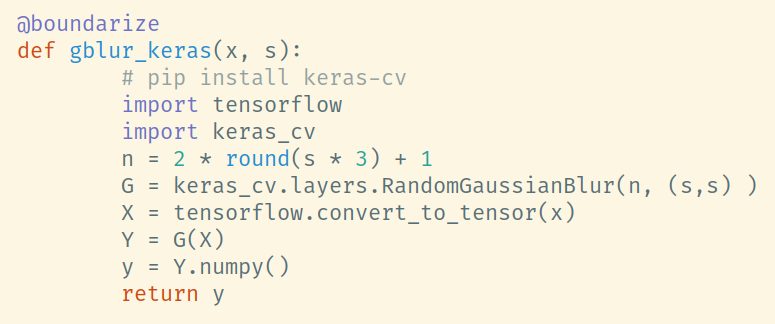
\includegraphics[width=\linewidth]{f/code_keras.png}}}
	\end{column}
\end{columns}

\vfill

\pause
Worked right away:
{\color{darkgreen}
pillow
vips
}

Required some hacking:
{\color{darkgreen}
opencv
skimage
scipy
torch
imagick
gmic
ffmpeg
julia:images
octave
tf:models
jax:pix
rust:image
}

Involved major hacking:
{\color{darkgreen}
krita
gimp
tf:keras
}

Not finished:
{\color{darkgreen}
darktable(hard!)
megawave
scilab
pnm
}

\end{frame}


% SLIDE context: previous 3 gttis that mention gaussian blur

% SLIDE "important distinction" image showin a good and a bad
% gaussian blur

% SLIDE gpt convo asking for gaussian blur

% SLIDE summary slide with all gaussian blurs that look mostly the same
% pillow, opencv, skimage, scipy, tfimage, torchvision, imagemagick, gimp, krita
% + one more!

% SLIDE xkcd 927 standards with "gaussian blurs" text overlaid

% SEC high-level comparisons (without looking at the results)

% SLIDE general principles of the comparison (images are arrays of numbers)

% SLIDE apis comparison (some highlights)

% SLIDE example with the "bad API chatgpt usage" with scipy.ndimage
%
%PYTHON import iio
%PYTHON from scipy.ndimage import gaussian_filter as G
%PYTHON x = iio.read("f/x.png")
%PYTHON iio.write("o/x_bndi_g1.png", G(x, sigma=1))
%PYTHON iio.write("o/x_bndi_g2.png", G(x, sigma=2))
%PYTHON iio.write("o/x_bndi_g7.png", G(x, sigma=7))
%PYTHON iio.write("o/x_ndi_g1.png", G(x, sigma=(1,1,0)))
%PYTHON iio.write("o/x_ndi_g2.png", G(x, sigma=(2,2,0)))
%PYTHON iio.write("o/x_ndi_g7.png", G(x, sigma=(7,7,0)))
\begin{frame}
EXAMPLE OF WRONG CODE GIVEN BY CHATGPT\\
======================================

	{\color{blue}
	from scipy.ndimage import gaussian\_filter as G
	}

	\begin{tabular}{llll}
		\tiny\color{blue}x&
		\tiny\color{blue}G(x, sigma=1)&
		\tiny\color{blue}G(x, sigma=2)&
		\tiny\color{blue}G(x, sigma=7)\\
		\includegraphics[width=0.23\linewidth]{f/x.png}&
		\includegraphics[width=0.23\linewidth]{o/x_bndi_g1.png}&
		\includegraphics[width=0.23\linewidth]{o/x_bndi_g2.png}&
		\includegraphics[width=0.23\linewidth]{o/x_bndi_g7.png}\\
	\end{tabular}

	\pause

	\begin{tabular}{llll}
		&
		\tiny\color{blue}G(x, sigma=(1,1,0) )&
		\tiny\color{blue}G(x, sigma=(2,2,0) )&
		\tiny\color{blue}G(x, sigma=(7,7,0) )\\
		\rule{0.23\linewidth}{0pt} &
		\includegraphics[width=0.23\linewidth]{o/x_ndi_g1.png}&
		\includegraphics[width=0.23\linewidth]{o/x_ndi_g2.png}&
		\includegraphics[width=0.23\linewidth]{o/x_ndi_g7.png}\\
	\end{tabular}
\end{frame}

\begin{frame}
EXAMPLE OF WRONG CODE GIVEN BY CHATGPT\\
======================================

	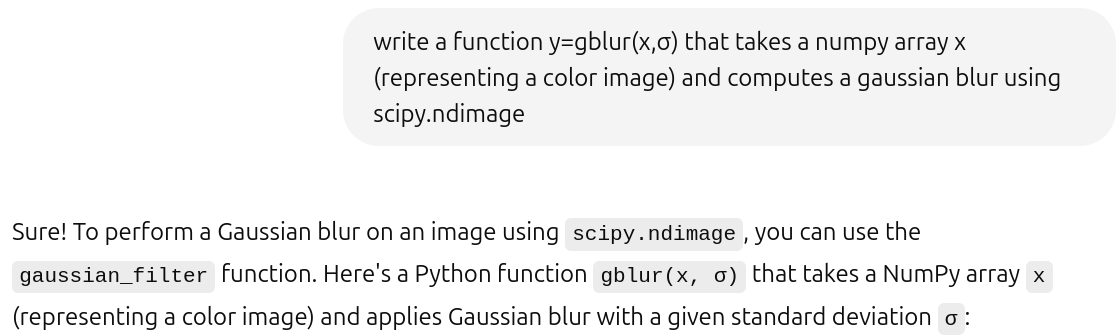
\includegraphics[width=0.7\linewidth]{f/gptshot1.png}

	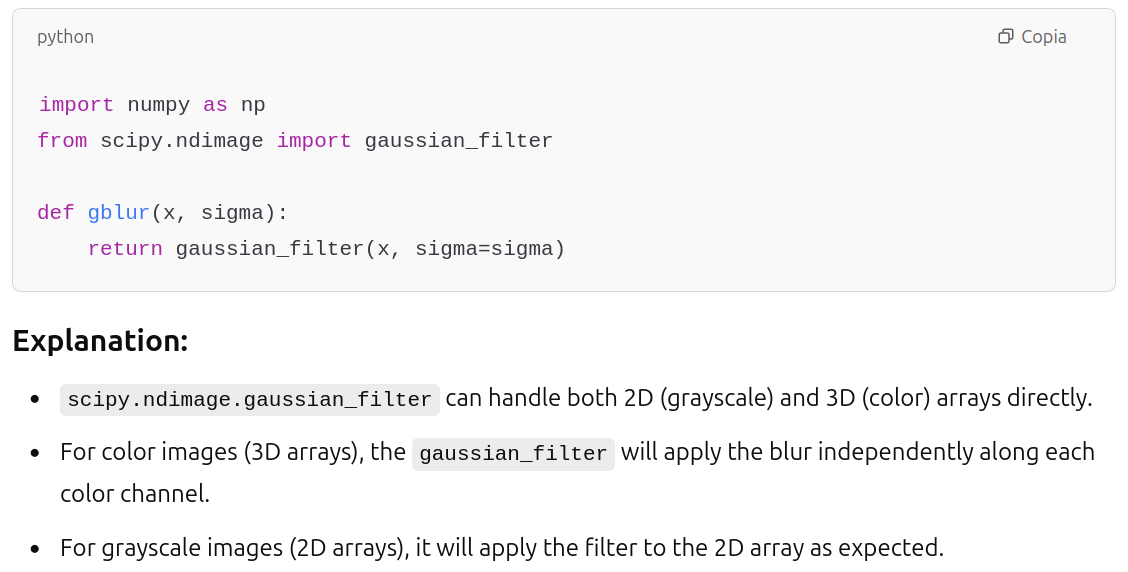
\includegraphics[width=0.7\linewidth]{f/gptshot2.png}
\end{frame}



% SECTIONING SLIDE
\begin{frame}%
\vfill
\begin{center}
\Huge
--2--\\External comparison
\end{center}
\vfill
\small
\centering
we just compare the results, without judging them
\end{frame}

% SLIDE running time comparison with graphs
\begin{frame}[fragile]
RUNNING TIME EVALUATION\\
=======================

Time to blur an image of size NxN with $\sigma=$s

\scriptsize
\begin{verbatim}
           N=1000,s=3   N=4000,s=3   N=1000,s=30    N=1000,s=100
borelli     0.27         3.18         0.26           0.26
torch       2.92         3.78         6.94          85.07
tfm         7.09        15.56        74.15           inf
keras       7.04         8.16         7.84           9.35
pix         0.89         1.91         1.50           3.00
pillow      0.22         0.58         0.26           0.23
scipy       0.31         0.77         0.59           1.20
opencv      0.20         0.35         0.31           0.47
skimage     0.32         0.76         0.59           1.14
vips        0.35         0.51         0.49           0.77
imagick     0.85        10.74        14.50           inf
gmic        0.50         0.84         0.52           0.47
ffmpeg      0.55         3.61         0.49           0.45
gimp        3.43        26.71         2.10           2.21
krita       2.00         8.29         2.15           2.49
rust        0.31         2.14         0.54           1.18
octave      0.61         2.91         5.93          49.00
julia       7.90         8.80         8.47           8.26
\end{verbatim}

\end{frame}

\begin{frame}
VISUAL COMPARISON\\
=================

N=1000 s=3

\tiny
\hspace*{-4em}\begin{tabular}{llllll}
	\includegraphics[width=0.15\linewidth]{o/r1000.png}&
	\includegraphics[width=0.15\linewidth]{o/r1000_g3_borelli.png}&
	\includegraphics[width=0.15\linewidth]{o/r1000_g3_torch.png}&
	\includegraphics[width=0.15\linewidth]{o/r1000_g3_tfm.png}&
	\includegraphics[width=0.15\linewidth]{o/r1000_g3_keras.png}&
	\includegraphics[width=0.15\linewidth]{o/r1000_g3_pix.png}\\
	 &
	{\bf\color{blue} borelli} &
	torchvision &
	tf:models &
	tf:keras &
	jax:pix \\
	%rust:image &
	%pillow \\
	&&&&&\\
	\includegraphics[width=0.15\linewidth]{o/r1000_g3_pillow.png}&
	\includegraphics[width=0.15\linewidth]{o/r1000_g3_scipy.png}&
	\includegraphics[width=0.15\linewidth]{o/r1000_g3_opencv.png}&
	\includegraphics[width=0.15\linewidth]{o/r1000_g3_skimage.png}&
	\includegraphics[width=0.15\linewidth]{o/r1000_g3_vips.png}&
	\includegraphics[width=0.15\linewidth]{o/r1000_g3_imagick.png}\\
	pillow &
	scipy:ndimage &
	opencv &
	skimage &
	vips &
	imagemagick \\
	&&&&&\\
	\includegraphics[width=0.15\linewidth]{o/r1000_g3_gmic.png}&
	\includegraphics[width=0.15\linewidth]{o/r1000_g3_gimp.png}&
	\includegraphics[width=0.15\linewidth]{o/r1000_g3_krita.png}&
	\includegraphics[width=0.15\linewidth]{o/r1000_g3_rust.png}&
	\includegraphics[width=0.15\linewidth]{o/r1000_g3_octave.png} &
	\includegraphics[width=0.15\linewidth]{o/r1000_g3_julia.png} \\
	gmic &
	gimp &
	krita &
	rust:image &
	octave &
	julia:Images \\
\end{tabular}
\end{frame}

\begin{frame}
VISUAL COMPARISON\\
=================

N=1000 s=30

\tiny
\hspace*{-4em}\begin{tabular}{llllll}
	\includegraphics[width=0.15\linewidth]{o/r1000.png}&
	\includegraphics[width=0.15\linewidth]{o/r1000_g30_borelli.png}&
	\includegraphics[width=0.15\linewidth]{o/r1000_g30_torch.png}&
	\includegraphics[width=0.15\linewidth]{o/r1000_g30_tfm.png}&
	\includegraphics[width=0.15\linewidth]{o/r1000_g30_keras.png}&
	\includegraphics[width=0.15\linewidth]{o/r1000_g30_pix.png}\\
	 &
	{\bf\color{blue} borelli} &
	torchvision &
	tf:models &
	tf:keras &
	jax:pix \\
	%rust:image &
	%pillow \\
	&&&&&\\
	\includegraphics[width=0.15\linewidth]{o/r1000_g30_pillow.png}&
	\includegraphics[width=0.15\linewidth]{o/r1000_g30_scipy.png}&
	\includegraphics[width=0.15\linewidth]{o/r1000_g30_opencv.png}&
	\includegraphics[width=0.15\linewidth]{o/r1000_g30_skimage.png}&
	\includegraphics[width=0.15\linewidth]{o/r1000_g30_vips.png}&
	\includegraphics[width=0.15\linewidth]{o/r1000_g30_imagick.png}\\
	pillow &
	scipy:ndimage &
	opencv &
	skimage &
	vips &
	imagemagick \\
	&&&&&\\
	\includegraphics[width=0.15\linewidth]{o/r1000_g30_gmic.png}&
	\includegraphics[width=0.15\linewidth]{o/r1000_g30_gimp.png}&
	\includegraphics[width=0.15\linewidth]{o/r1000_g30_krita.png}&
	\includegraphics[width=0.15\linewidth]{o/r1000_g30_rust.png}&
	\includegraphics[width=0.15\linewidth]{o/r1000_g30_octave.png} &
	\includegraphics[width=0.15\linewidth]{o/r1000_g30_julia.png} \\
	gmic &
	gimp &
	krita &
	rust:image &
	octave &
	julia:Images \\
\end{tabular}
\end{frame}


\begin{frame}
VISUAL COMPARISON\\
=================

N=1000 s=100

\tiny
\hspace*{-4em}\begin{tabular}{llllll}
	\includegraphics[width=0.15\linewidth]{o/r1000.png}&
	\includegraphics[width=0.15\linewidth]{o/r1000_g100_borelli.png}&
	\includegraphics[width=0.15\linewidth]{o/r1000_g100_torch.png}&
	&%\includegraphics[width=0.15\linewidth]{o/r1000_g100_tfm.png}
	\includegraphics[width=0.15\linewidth]{o/r1000_g100_keras.png}&
	\includegraphics[width=0.15\linewidth]{o/r1000_g100_pix.png}\\
	 &
	{\bf\color{blue} borelli} &
	torchvision &
	tf:models &
	tf:keras &
	jax:pix \\
	%rust:image &
	%pillow \\
	&&&&&\\
	\includegraphics[width=0.15\linewidth]{o/r1000_g100_pillow.png}&
	\includegraphics[width=0.15\linewidth]{o/r1000_g100_scipy.png}&
	\includegraphics[width=0.15\linewidth]{o/r1000_g100_opencv.png}&
	\includegraphics[width=0.15\linewidth]{o/r1000_g100_skimage.png}&
	\includegraphics[width=0.15\linewidth]{o/r1000_g100_vips.png}&
	\\ %\includegraphics[width=0.15\linewidth]{o/r1000_g100_imagick.png}\\
	pillow &
	scipy:ndimage &
	opencv &
	skimage &
	vips &
	imagemagick \\
	&&&&&\\
	\includegraphics[width=0.15\linewidth]{o/r1000_g100_gmic.png}&
	\includegraphics[width=0.15\linewidth]{o/r1000_g100_gimp.png}&
	\includegraphics[width=0.15\linewidth]{o/r1000_g100_krita.png}&
	\includegraphics[width=0.15\linewidth]{o/r1000_g100_rust.png}&
	\includegraphics[width=0.15\linewidth]{o/r1000_g100_octave.png} &
	\includegraphics[width=0.15\linewidth]{o/r1000_g100_julia.png} \\
	gmic &
	gimp &
	krita &
	rust:image &
	octave &
	julia:Images \\
\end{tabular}

\end{frame}

\begin{frame}
RUNNING TIME EVALUATION\\
=======================

table with running times of each algorithm with three columns\\
- 1000x1000 sigma 3\\
- 5000x5000 sigma 3\\
- 1000x1000 sigma 300

graph with runing time as a function of image size, for constant sigma (show three representative behaviors)

graph with running time as a function of sigma, for images of the same size
	(show three representative behaviors)
\end{frame}

% SLIDE cosine similarity distance table
\begin{frame}
NUMERICAL SIMILARITY BETWEEN THE RESULTS\\
========================================

\scriptsize
	\hspace*{-2em}%
	\begin{tabular}{ll}
		\includegraphics[width=0.51\linewidth]{summary_bdef.png}&
		\only<2>{
			\includegraphics[width=0.51\linewidth]{summary_bp.png}}
		\\
		\only<1>{\hspace*{10em}RMSE}\only<2>{RMSE (default boundary conditions)} &
		\only<2>{RMSE (periodic boundary conditions)}
	\end{tabular}

\vfill

LEGEND: black=0, white=20
\end{frame}


\begin{frame}
VISUAL COMPARISON OF THE DIFFERENCES\\
====================================

\tiny
\hspace*{-4em}\begin{tabular}{llllll}
	%\includegraphics[width=0.15\linewidth]{o/.png}
	&
	\includegraphics[width=0.15\linewidth]{o/d_borelli_borelli.png}&
	\includegraphics[width=0.15\linewidth]{o/d_borelli_torch.png}&
	\includegraphics[width=0.15\linewidth]{o/d_borelli_tfm.png}&
	\includegraphics[width=0.15\linewidth]{o/d_borelli_keras.png}&
	\includegraphics[width=0.15\linewidth]{o/d_borelli_pix.png}\\
	 &
	{\bf\color{blue} borelli} &
	torchvision &
	tf:models &
	tf:keras &
	jax:pix \\
	%rust:image &
	%pillow \\
	&&&&&\\
	\includegraphics[width=0.15\linewidth]{o/d_borelli_pillow.png}&
	\includegraphics[width=0.15\linewidth]{o/d_borelli_scipy.png}&
	\includegraphics[width=0.15\linewidth]{o/d_borelli_opencv.png}&
	\includegraphics[width=0.15\linewidth]{o/d_borelli_skimage.png}&
	\includegraphics[width=0.15\linewidth]{o/d_borelli_vips.png}&
	\includegraphics[width=0.15\linewidth]{o/d_borelli_imagick.png}\\
	pillow &
	scipy:ndimage &
	opencv &
	skimage &
	vips &
	imagemagick \\
	&&&&&\\
	\includegraphics[width=0.15\linewidth]{o/d_borelli_gmic.png}&
	\includegraphics[width=0.15\linewidth]{o/d_borelli_gimp.png}&
	\includegraphics[width=0.15\linewidth]{o/d_borelli_krita.png}&
	\includegraphics[width=0.15\linewidth]{o/d_borelli_rust.png}&
	\includegraphics[width=0.15\linewidth]{o/d_borelli_octave.png} &
	\includegraphics[width=0.15\linewidth]{o/d_borelli_julia.png} \\
	gmic &
	gimp &
	krita &
	rust:image &
	octave &
	julia:Images \\
\end{tabular}

\end{frame}

\begin{frame}
VISUAL COMPARISON OF THE DIFFERENCES\\
====================================

\tiny
\hspace*{-4em}\begin{tabular}{llllll}
	%\includegraphics[width=0.15\linewidth]{o/.png}
	&
	\includegraphics[width=0.15\linewidth]{o/d_opencv_borelli.png}&
	\includegraphics[width=0.15\linewidth]{o/d_opencv_torch.png}&
	\includegraphics[width=0.15\linewidth]{o/d_opencv_tfm.png}&
	\includegraphics[width=0.15\linewidth]{o/d_opencv_keras.png}&
	\includegraphics[width=0.15\linewidth]{o/d_opencv_pix.png}\\
	 &
	{\bf\color{blue} borelli} &
	torchvision &
	tf:models &
	tf:keras &
	jax:pix \\
	%rust:image &
	%pillow \\
	&&&&&\\
	\includegraphics[width=0.15\linewidth]{o/d_opencv_pillow.png}&
	\includegraphics[width=0.15\linewidth]{o/d_opencv_scipy.png}&
	\includegraphics[width=0.15\linewidth]{o/d_opencv_opencv.png}&
	\includegraphics[width=0.15\linewidth]{o/d_opencv_skimage.png}&
	\includegraphics[width=0.15\linewidth]{o/d_opencv_vips.png}&
	\includegraphics[width=0.15\linewidth]{o/d_opencv_imagick.png}\\
	pillow &
	scipy:ndimage &
	opencv &
	skimage &
	vips &
	imagemagick \\
	&&&&&\\
	\includegraphics[width=0.15\linewidth]{o/d_opencv_gmic.png}&
	\includegraphics[width=0.15\linewidth]{o/d_opencv_gimp.png}&
	\includegraphics[width=0.15\linewidth]{o/d_opencv_krita.png}&
	\includegraphics[width=0.15\linewidth]{o/d_opencv_rust.png}&
	\includegraphics[width=0.15\linewidth]{o/d_opencv_octave.png} &
	\includegraphics[width=0.15\linewidth]{o/d_opencv_julia.png} \\
	gmic &
	gimp &
	krita &
	rust:image &
	octave &
	julia:Images \\
\end{tabular}

\end{frame}


\begin{frame}
VISUAL COMPARISON OF THE DIFFERENCES\\
====================================

\tiny
\hspace*{-4em}\begin{tabular}{llllll}
	%\includegraphics[width=0.15\linewidth]{o/.png}
	&
	\includegraphics[width=0.15\linewidth]{o/d_torch_borelli.png}&
	\includegraphics[width=0.15\linewidth]{o/d_torch_torch.png}&
	\includegraphics[width=0.15\linewidth]{o/d_torch_tfm.png}&
	\includegraphics[width=0.15\linewidth]{o/d_torch_keras.png}&
	\includegraphics[width=0.15\linewidth]{o/d_torch_pix.png}\\
	 &
	{\bf\color{blue} borelli} &
	torchvision &
	tf:models &
	tf:keras &
	jax:pix \\
	%rust:image &
	%pillow \\
	&&&&&\\
	\includegraphics[width=0.15\linewidth]{o/d_torch_pillow.png}&
	\includegraphics[width=0.15\linewidth]{o/d_torch_scipy.png}&
	\includegraphics[width=0.15\linewidth]{o/d_torch_opencv.png}&
	\includegraphics[width=0.15\linewidth]{o/d_torch_skimage.png}&
	\includegraphics[width=0.15\linewidth]{o/d_torch_vips.png}&
	\includegraphics[width=0.15\linewidth]{o/d_torch_imagick.png}\\
	pillow &
	scipy:ndimage &
	opencv &
	skimage &
	vips &
	imagemagick \\
	&&&&&\\
	\includegraphics[width=0.15\linewidth]{o/d_torch_gmic.png}&
	\includegraphics[width=0.15\linewidth]{o/d_torch_gimp.png}&
	\includegraphics[width=0.15\linewidth]{o/d_torch_krita.png}&
	\includegraphics[width=0.15\linewidth]{o/d_torch_rust.png}&
	\includegraphics[width=0.15\linewidth]{o/d_torch_octave.png} &
	\includegraphics[width=0.15\linewidth]{o/d_torch_julia.png} \\
	gmic &
	gimp &
	krita &
	rust:image &
	octave &
	julia:Images \\
\end{tabular}

\end{frame}

% SLIDE comparison of boundary conditions
\begin{frame}
BOUNDARY CONDITIONS\\
===================

%MAKE all: o/bd_0.png o/bd_p.png o/bd_n.png o/bd_s.png
%MAKE o/bd_0.png : f/x.png ; GETPIXEL=0 plambda zero:1144x1144 $^ 'x y(-286,-286)' |downsa v 3 - $@
%MAKE o/bd_p.png : f/x.png ; GETPIXEL=periodic plambda zero:1144x1144 $^ 'x y(-286,-286)' |downsa v 3 - $@
%MAKE o/bd_n.png : f/x.png ; GETPIXEL=nearest plambda zero:1144x1144 $^ 'x y(-286,-286)' |downsa v 3 - $@
%MAKE o/bd_s.png : f/x.png ; GETPIXEL=symmetric plambda zero:1144x1144 $^ 'x y(-286,-286)' |downsa v 3 - $@

\hspace*{-1.5em}\begin{tabular}{llll}
	\includegraphics[width=0.24\linewidth]{o/bd_0.png}&
	\includegraphics[width=0.24\linewidth]{o/bd_p.png}&
	\includegraphics[width=0.24\linewidth]{o/bd_n.png}&
	\includegraphics[width=0.24\linewidth]{o/bd_s.png}\\
	constant & periodic & nearest & symmetric
\end{tabular}

- each of the 18 implementations uses its own default

- not all of them give all the choices to the user

- {\color{blue}gblurs.py} allows to set the B.C. independently

\end{frame}



% SECTIONING SLIDE
\begin{frame}%
\vfill
\begin{center}
\Huge
--3--\\Who wins?
\end{center}
\vfill
\small
\centering
	{{\bf we do!}
	(by carefully defining the criteria so that we win)
	}
\end{frame}



% recall gaussian noise and gaussian blur
\begin{frame}[noframenumbering]

	\vfill
\begin{center}
{\color{red}\huge
	WARNING!

	important distinction:
}
\end{center}
	\vfill

%SCRIPT plambda f/x.png "randg randg randg rgb 60 * +" -o o/gnoise.png
%SCRIPT blur g 8  f/x.png o/gblur.png
%SCRIPT blur s 20  f/x.png o/sblur.png

\begin{tabular}{cc}%c}
	%\includegraphics[width=0.3\linewidth]{photos/gbarbsquare.png}&
	\includegraphics[width=0.46\linewidth]{o/gblur.png}&
	\includegraphics[width=0.46\linewidth]{o/gnoise.png}\\
	%input image &
	\color{red} gaussian blur &%$\sigma=30$ &
	\color{red} gaussian noise %/$\sigma=10$ \\
\end{tabular}
	\vfill
\end{frame}

\begin{frame}[noframenumbering]

	\vfill
\begin{center}
{\color{blue}\huge
	WARNING!

	important distinction:
}
\end{center}
	\vfill

\begin{tabular}{cc}%c}
	%\includegraphics[width=0.3\linewidth]{photos/gbarbsquare.png}&
	\includegraphics[width=0.46\linewidth]{o/gblur.png}&
	\includegraphics[width=0.46\linewidth]{o/sblur.png}\\
	%input image &
	\color{blue} gaussian blur &%$\sigma=30$ &
	\color{blue} non-gaussian blur %/$\sigma=10$ \\
\end{tabular}
	\vfill
\end{frame}

\begin{frame}
THE GAUSSIAN KERNEL IN~$\R^2$\\
=============================

	{\bf Definition:}\\[.3em]
$G_\sigma(x)=\frac1{2\pi\sigma}e^{-\|x\|^2/2\sigma^2}$
	{\color{lightgray}\small
	(acting by convolution
	on~$f:\R^2\to\R$)
%$G_\sigma f := G_\sigma * f$
	}

	{\bf Properties:}\\[.3em]
$\widehat{G_\sigma}(\xi)=e^{-\sigma^2\|\xi\|^2/2}$
	{$\quad$\color{lightgray}(spectral response)}\\[.3em]
$G_\sigma G_\mu=G_{\sqrt{\sigma^2+\mu^2}}$
	{$\quad$\color{lightgray}(semigroup)}\\[.3em]
$G_\sigma T_a=T_a G_{\sigma}$
	{$\quad$\color{lightgray}(shift-invariance, for $T_af(x)=f(x-a)$)}\\[.3em]
$G_\sigma H_\lambda=H_\lambda G_{\lambda\sigma}$
	{$\quad$\color{lightgray}(scaling, for $H_\lambda f(x)=f(x/\lambda)$)}\\[.3em]
	$G_\sigma f(x) =f(x) + \frac{\sigma^2}2\Delta f(x)+O(\sigma^3)$
	{$\quad$\color{lightgray}(laplacian consistency)}\\[.3em]
	$\displaystyle\lim_{\sigma\to\infty}G_\sigma f =\mathrm{avg}(f)$
	{$\quad$\color{lightgray}(mass conservation)}\\[.3em]

	\vfill
	\pause

	\color{blue}
	{\bf Discrete case:}
	{\color{cyan}
	for~$f:\Z^2\to\R$ or $f:\Z^2/\left(W\Z\times H\Z\right)\quad$}\\[.3em]
	$\mathbf{G}_\sigma := S_1 G_\sigma \mathbf{I}_1$
	{$\quad$\color{lightgray}(with $\mathbf{I}_1$=Shannon interp. and~$S_1=$sampling)}\\[.3em]

\end{frame}

% SEC the gaussian semigroup: definition, properties, discrete versions
\begin{frame}
WHAT IS THE BEST METHOD? (THEORETICAL ANSWER)\\
=============================================

	{\bf Proposition.} (Borelli wins)\\
	The algorithm {\color{blue}gblur\_borelli} is the only one that satisfies
	all the required numerical properties of the discrete Gaussian semigroup.

	\vfill

	$\mathbf{G}_\sigma := S_1 G_\sigma \mathbf{I}_1$

	$\mathbf{G}_\sigma\mathbf{G}_\mu =
	(S_1 G_\sigma {\color{red}\mathbf{I}_1})
	({\color{red}S_1} G_\mu \mathbf{I}_1)
	=
	S_1 G_\sigma G_\mu \mathbf{I}_1=\cdots
	$

	\vfill
	\begin{center}
		{%
			\setlength{\fboxsep}{0pt}%
			\setlength{\fboxrule}{0.5pt}%
			\fbox{\includegraphics[width=0.9\linewidth]{f/gblur_borelli.png}}
		}
	\end{center}
\end{frame}

\begin{frame}
WHAT IS THE BEST METHOD? (NUMERICAL ANSWER)\\
===========================================

numerical verification of the semigroup property

numerical verification of limiting cases

numerical verification of energy conservation

numerical verification of linearity

numerical verification of laplacian-consistency

numerical verification of heat equation
\end{frame}


\begin{frame}
NUMERICAL TEST OF THE SEMIGROUP PROPERTY\\
========================================

$G_3 G_4 u - G_5 u$

\tiny
\hspace*{-4em}\begin{tabular}{llllll}
	%\includegraphics[width=0.15\linewidth]{o/.png}
	&
	\includegraphics[width=0.15\linewidth]{o/gd_3_4_5_borelli.png}&
	\includegraphics[width=0.15\linewidth]{o/gd_3_4_5_torch.png}&
	\includegraphics[width=0.15\linewidth]{o/gd_3_4_5_tfm.png}&
	\includegraphics[width=0.15\linewidth]{o/gd_3_4_5_keras.png}&
	\includegraphics[width=0.15\linewidth]{o/gd_3_4_5_pix.png}\\
	 &
	{\bf\color{blue} borelli} &
	torchvision &
	tf:models &
	tf:keras &
	jax:pix \\
	%rust:image &
	%pillow \\
	&&&&&\\
	\includegraphics[width=0.15\linewidth]{o/gd_3_4_5_pillow.png}&
	\includegraphics[width=0.15\linewidth]{o/gd_3_4_5_scipy.png}&
	\includegraphics[width=0.15\linewidth]{o/gd_3_4_5_opencv.png}&
	\includegraphics[width=0.15\linewidth]{o/gd_3_4_5_skimage.png}&
	\includegraphics[width=0.15\linewidth]{o/gd_3_4_5_vips.png}&
	\includegraphics[width=0.15\linewidth]{o/gd_3_4_5_imagick.png}\\
	pillow &
	scipy:ndimage &
	opencv &
	skimage &
	vips &
	imagemagick \\
	&&&&&\\
	\includegraphics[width=0.15\linewidth]{o/gd_3_4_5_gmic.png}&
	\includegraphics[width=0.15\linewidth]{o/gd_3_4_5_gimp.png}&
	\includegraphics[width=0.15\linewidth]{o/gd_3_4_5_krita.png}&
	\includegraphics[width=0.15\linewidth]{o/gd_3_4_5_rust.png}&
	\includegraphics[width=0.15\linewidth]{o/gd_3_4_5_octave.png} &
	\includegraphics[width=0.15\linewidth]{o/gd_3_4_5_julia.png} \\
	gmic &
	gimp &
	krita &
	rust:image &
	octave &
	julia:Images \\
\end{tabular}

\end{frame}



\begin{frame}
NUMERICAL TEST OF THE SEMIGROUP PROPERTY\\
========================================

$G_5 G_{12} u - G_{13} u$

\tiny
\hspace*{-4em}\begin{tabular}{llllll}
	%\includegraphics[width=0.15\linewidth]{o/.png}
	&
	\includegraphics[width=0.15\linewidth]{o/gd_5_12_13_borelli.png}&
	\includegraphics[width=0.15\linewidth]{o/gd_5_12_13_torch.png}&
	\includegraphics[width=0.15\linewidth]{o/gd_5_12_13_tfm.png}&
	\includegraphics[width=0.15\linewidth]{o/gd_5_12_13_keras.png}&
	\includegraphics[width=0.15\linewidth]{o/gd_5_12_13_pix.png}\\
	 &
	{\bf\color{blue} borelli} &
	torchvision &
	tf:models &
	tf:keras &
	jax:pix \\
	%rust:image &
	%pillow \\
	&&&&&\\
	\includegraphics[width=0.15\linewidth]{o/gd_5_12_13_pillow.png}&
	\includegraphics[width=0.15\linewidth]{o/gd_5_12_13_scipy.png}&
	\includegraphics[width=0.15\linewidth]{o/gd_5_12_13_opencv.png}&
	\includegraphics[width=0.15\linewidth]{o/gd_5_12_13_skimage.png}&
	\includegraphics[width=0.15\linewidth]{o/gd_5_12_13_vips.png}&
	\includegraphics[width=0.15\linewidth]{o/gd_5_12_13_imagick.png}\\
	pillow &
	scipy:ndimage &
	opencv &
	skimage &
	vips &
	imagemagick \\
	&&&&&\\
	\includegraphics[width=0.15\linewidth]{o/gd_5_12_13_gmic.png}&
	\includegraphics[width=0.15\linewidth]{o/gd_5_12_13_gimp.png}&
	\includegraphics[width=0.15\linewidth]{o/gd_5_12_13_krita.png}&
	\includegraphics[width=0.15\linewidth]{o/gd_5_12_13_rust.png}&
	\includegraphics[width=0.15\linewidth]{o/gd_5_12_13_octave.png} &
	\includegraphics[width=0.15\linewidth]{o/gd_5_12_13_julia.png} \\
	gmic &
	gimp &
	krita &
	rust:image &
	octave &
	julia:Images \\
\end{tabular}

\end{frame}

% SLIDE verification of the semi-group property

% SLIDE verification of the linearity, translation and 90-degree rotation props

% SLIDE verification of laplacian-consistency

% SLIDE verification of limiting cases (σ=0:identity, σ=∞:average)

% SLIDE summary table

% SLIDE ymscript's implementation

% SLIDE unified API call

% SLIDE (small python rant about dependencies and global imports)

% SLIDE notebook show

\begin{frame}
CAVEATS\\
=======

The problem of~$\gamma$:
$\color{red}G_\sigma\left(u^\gamma\right) \neq \left(G_\sigma u\right)^\gamma$

%MAKE all: o/gamma_bands.png o/gamma_constant.png
%MAKE o/gamma_bands.png:    ;plambda zero:200x200 "-1 :i ^ 1 + 127 *" -o $@
%MAKE o/gamma_constant.png: ;plambda zero:200x200 "127" -o $@

\begin{tabular}{ll}
	\includegraphics[width=0.46\linewidth]{o/gamma_bands.png}&
	\includegraphics[width=0.46\linewidth]{o/gamma_constant.png}\\
	$u(i,j) = 127\left(1+(-1)^i\right)$ &
	$u(i,j) = 127$
\end{tabular}

\vfill

\pause
	\color{red}{\bf Corollary.} Gaussian blur is IMPOSSIBLE.

\end{frame}

% 25. colophon: source code of the article and the presentation
\begin{frame}
COLOPHON\\
========

	\begin{center}
		{%
			\setlength{\fboxsep}{0pt}%
			\setlength{\fboxrule}{0.5pt}%
			\fbox{\includegraphics[width=\linewidth]{o/gblur_borelli.png}}
		}
	\end{center}

\end{frame}






\end{document}


% vim:sw=2 ts=2 :
